\subsection{\texorpdfstring{$y''+(ax^4+bx^3+cx^2+dx+e)y = 
0$}{y''-(ax4+bx3+cx2+dx+e)y = 0}}

Auch ein Polynom $4$-ten Grades stellt kein Problem mehr dar. Einfach in die 
Formel (\ref{eq:wellen:allgemeineak}) eingesetzt, ergibt

\begin{equation*}
	\begin{split}
		a_k &= -\frac{1}{k(k-1)} (aa_{k-2-4} + 
		ba_{k-2-3} + ca_{k-2-2} + da_{k-2-1} +ea_{k-2-0})
		\\
		&= -\frac{1}{k(k-1)} (aa_{k-6} + ba_{k-5} + 
		ca_{k-4} + da_{k-3} +ea_{k-2}), \qquad a_{k<0} = 0
	\end{split}
\end{equation*}

Auch hier k"onnen wir in der Abbildung \ref{fig:wellen:poly4-dgl} die 
"Uberg"ange zwischen Sinus und Cosinus bei positiven und Sinus Hyperbolicus und 
Cosinus Hyperbolicus bei negativen Polynoml"osungen deutlich sehen.

\begin{figure}
	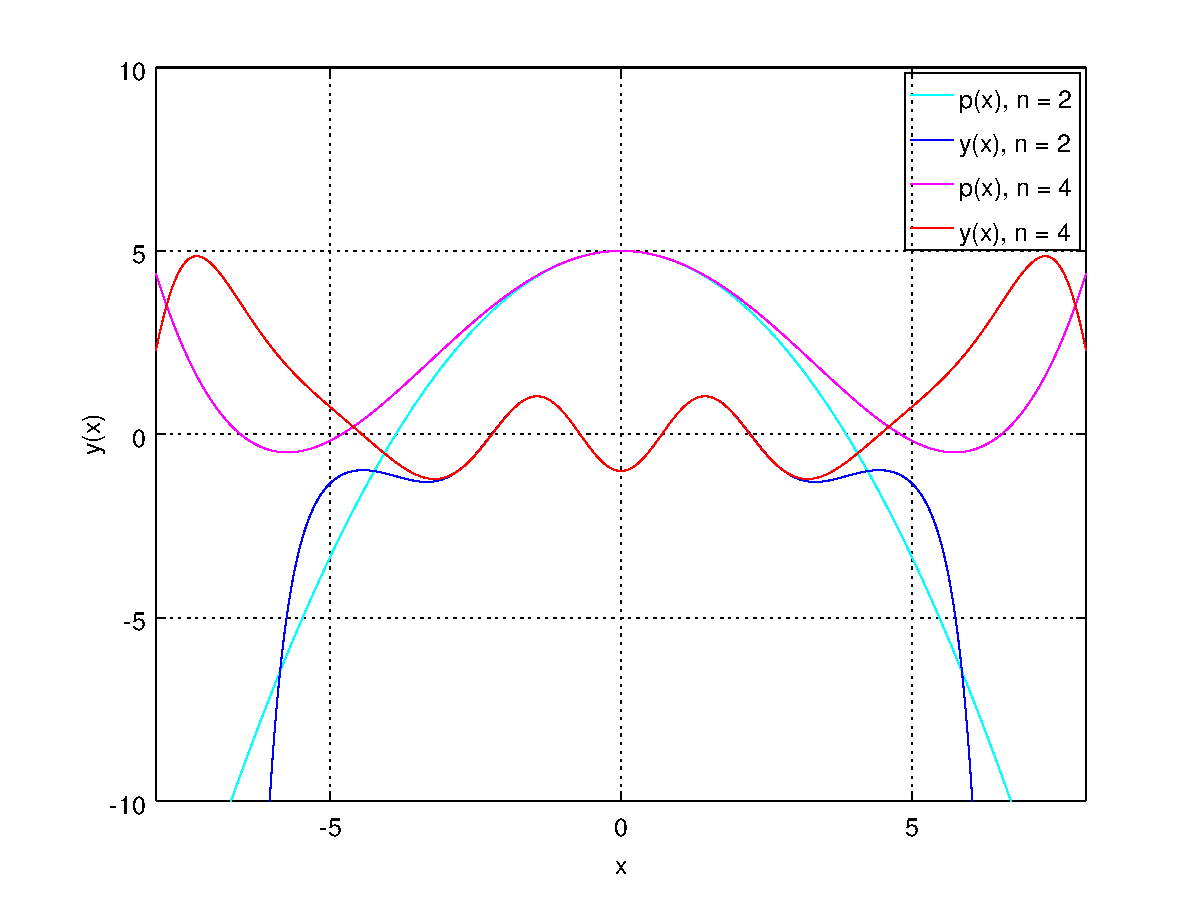
\includegraphics[scale=0.65]{./wellen/images/allgemein/n4.pdf}
	\caption{L"osung Polynom 4-ten Grades}
	\label{fig:wellen:poly4-dgl}
\end{figure}